\subsection{Гравитационное линзирование}
\term{Гравитационное линзирование}~--- эффект, связанный с искривлением пути
\begin{wrapfigure}[9]{l}{0.35\tw}
	\centering
	\vspace{-1pc}
	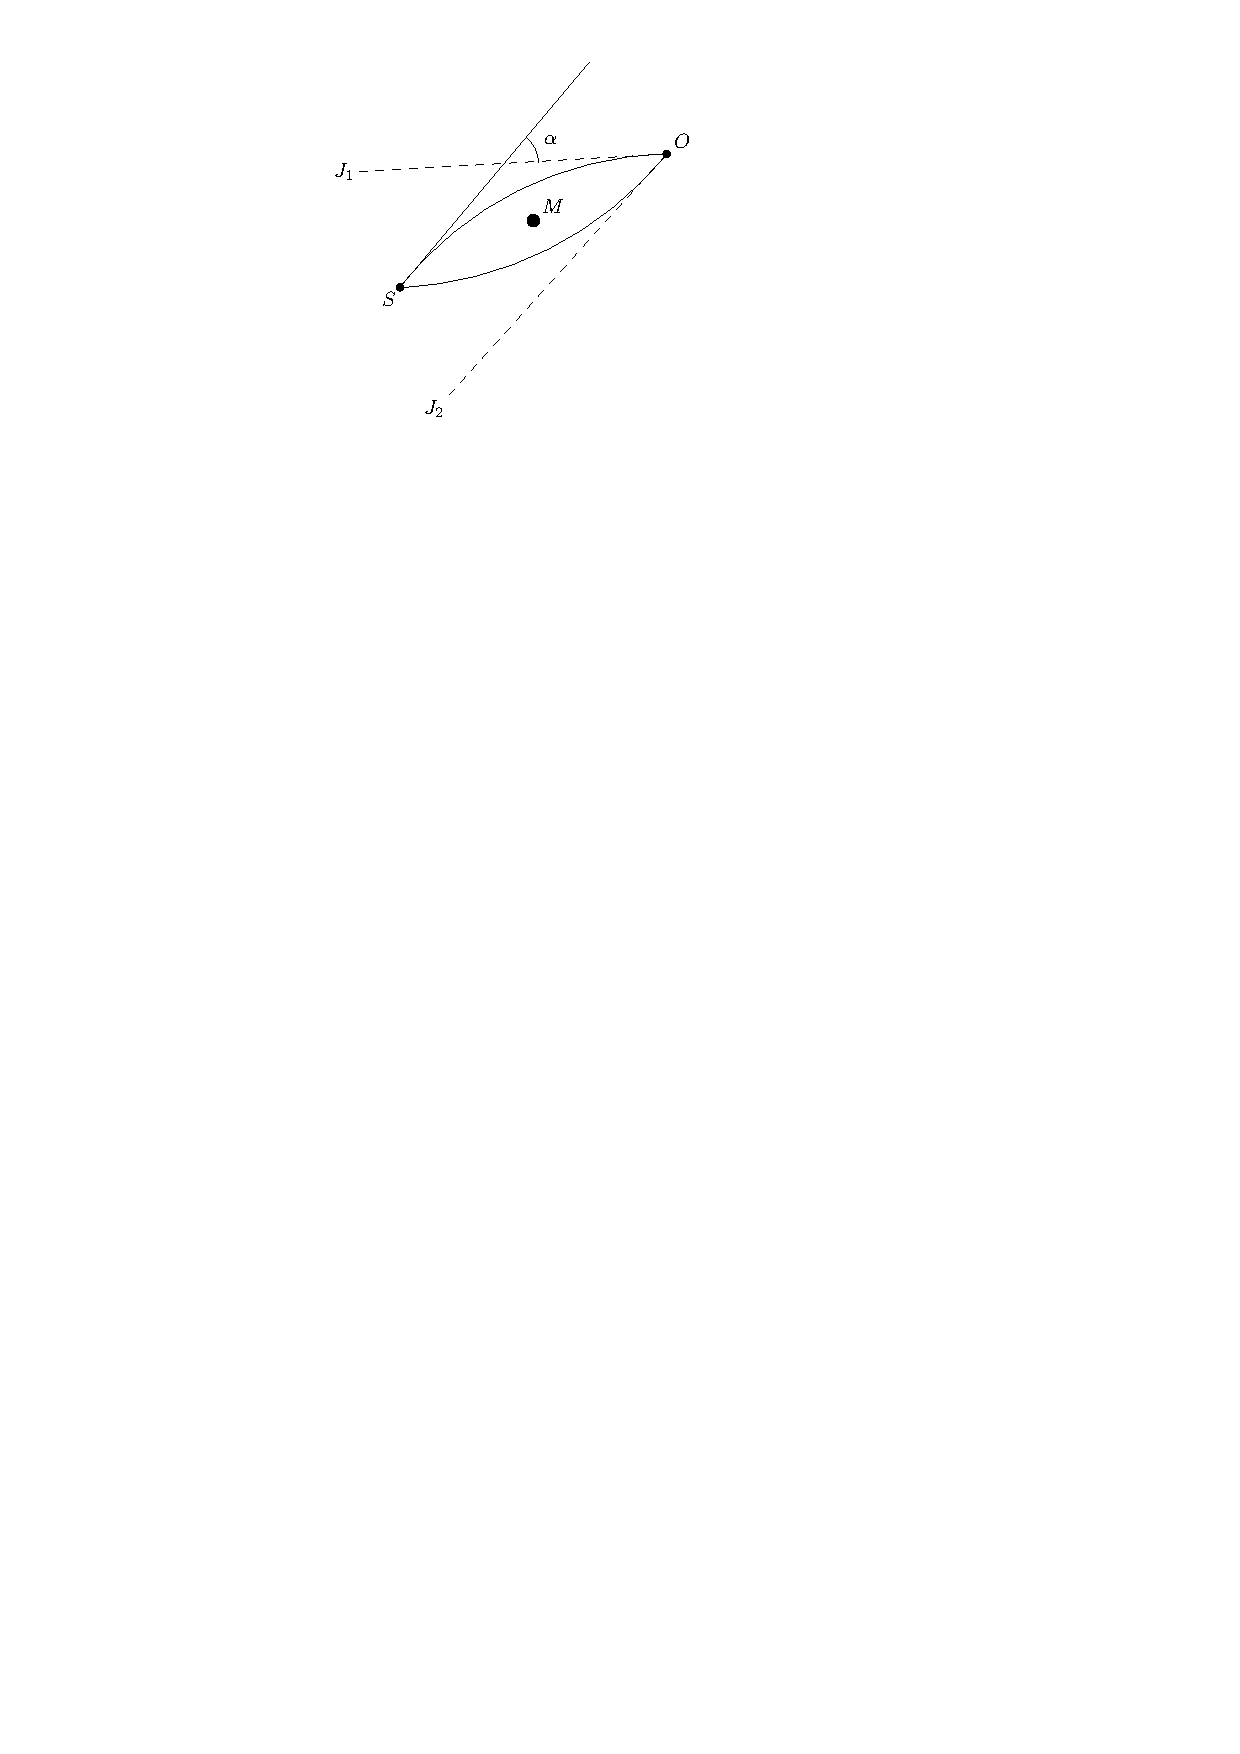
\includegraphics[width=0.35\tw]{grav-lens}
 	\caption{Гравитационное линзирование}
	\label{grav-lens}
\end{wrapfigure}
распространения электромагнитного излучения гравитационным полем массивного тела или системы тел (галактик, скопления галактик, скопления тёмной материи).

На Рис.\,\ref{grav-lens} показано, как происходит гравитационное линзирование: $S$~--- источник электромагнитных волн, $O$~--- наблюдатель, $J_1$ и $J_2$~--- видимые положения источника, $M$~--- массивное тело массы $M$ и радиуса $R$.

Для угла преломления лучей $\alpha$ в ходе гравитационного линзирования справедлива формула
\begin{equation}
	\alpha = \frac{4 G M}{R c^2}.
\end{equation}